\chapter{Практичні результати}

У четвертому розділі представлено практичні результати
застосування алгоритму дифузії з сегментацією
та без із зазначенням вхідних даних.

\section{Результати експериментів}

Вихідні зображення для побудови карти глибин
за допомогою описаних алгоритмів були взяті з набору стереопар,
зроблених в Мідлберійському коледжі в 2001~\cite{middlebury:ds:2001},
2003~\cite{middlebury:ds:2003}
та 2006~\cite{middlebury:ds:2006:1}~\cite{middlebury:ds:2006:2} роках.
На рисунку \ref{fig:stereopair} наведені ліві та праві зображення зі стереопар,
для яких будувались карти глибин в даному розділі дисертації.

\begin{figure}[h]
\centering
    \begin{subfigure}[t]{0.32\textwidth}
        \centering
        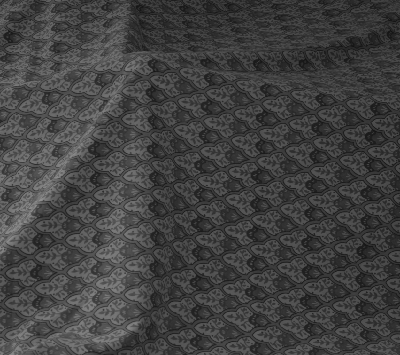
\includegraphics[width=\textwidth]{images/cloth_left}
    \end{subfigure}
    \hfill
    \begin{subfigure}[t]{0.32\textwidth}
        \centering
        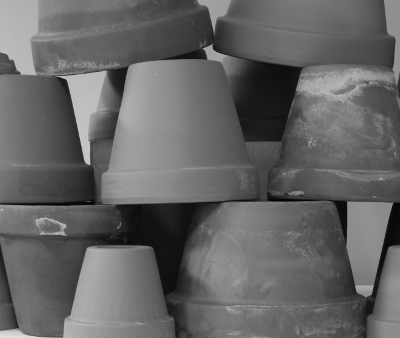
\includegraphics[width=\textwidth]{images/pots_left}
    \end{subfigure}
    \hfill
    \begin{subfigure}[t]{0.32\textwidth}
        \centering
        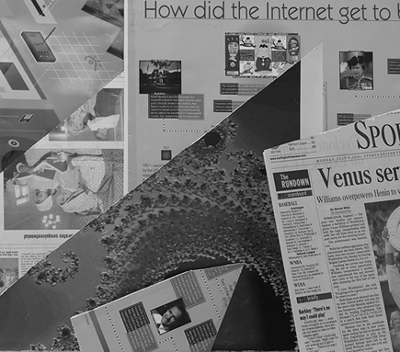
\includegraphics[width=\textwidth]{images/poster_left}
    \end{subfigure}
    \vskip\baselineskip
    \begin{subfigure}[t]{0.32\textwidth}
        \centering
        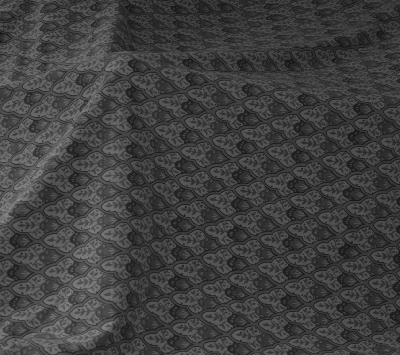
\includegraphics[width=\textwidth]{images/cloth_right}
        \caption{Тканина (Cloth1), $400 \times 355$ пікселів}
    \end{subfigure}
    \hfill
    \begin{subfigure}[t]{0.32\textwidth}
        \centering
        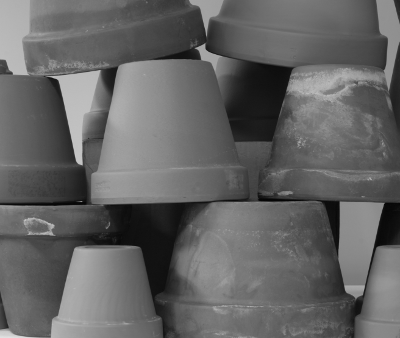
\includegraphics[width=\textwidth]{images/pots_right}
        \caption{Квіткові горщики (Flowerpots), $400 \times 338$ пікселів}
    \end{subfigure}
    \hfill
    \begin{subfigure}[t]{0.32\textwidth}
        \centering
        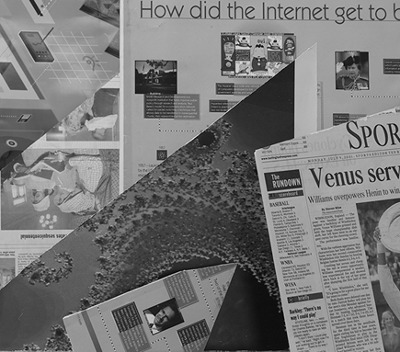
\includegraphics[width=\textwidth]{images/poster_right}
        \caption{Плакат (Poster), $400 \times 352$ пікселів}
    \end{subfigure}
    \caption{Зображення стереопар,
             для яких будувались карти глибин в цьому розділі.
             Перший рядок містить ліві зображення, другий~---~праві}
    \label{fig:stereopair}
\end{figure}

На рисунку \ref{fig:result:pixel} зображені карти глибин,
отримані за допомогою алгоритму дифузії,
де кожній долі графу відповідає один піксель,
як описано в другому розділі дисертації.
Для кожного зображення вказано кількість ітерацій, зроблений алгоритмом дифузії,
час виконання всіх ітерацій, а також кількість міток $\left| D \right|$ в графі.

\begin{figure}[h]
\centering
    \begin{subfigure}[t]{0.32\textwidth}
        \centering
        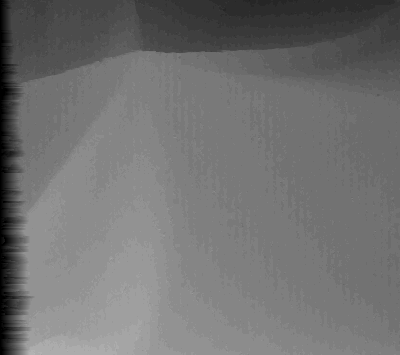
\includegraphics[width=\textwidth]{images/cloth_pixel_based_stereo}
        \caption{$2'400$ ітерацій, $5$ годин $40$ хвилин, $\left| D \right| = 40$}
        \label{fig:cloth:pixel}
    \end{subfigure}
    \hfill
    \begin{subfigure}[t]{0.32\textwidth}
        \centering
        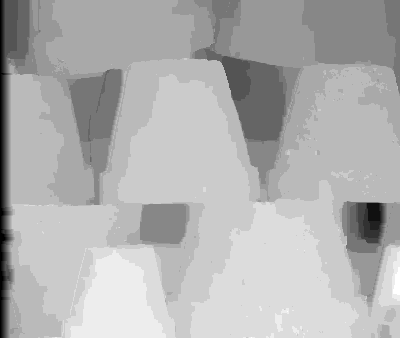
\includegraphics[width=\textwidth]{images/pots_pixel_based_stereo}
        \caption{$2'800$ ітерацій, $1$ година $20$ хвилин, $\left| D \right| = 16$}
        \label{fig:flowerpots:pixel}
    \end{subfigure}
    \hfill
    \begin{subfigure}[t]{0.32\textwidth}
        \centering
        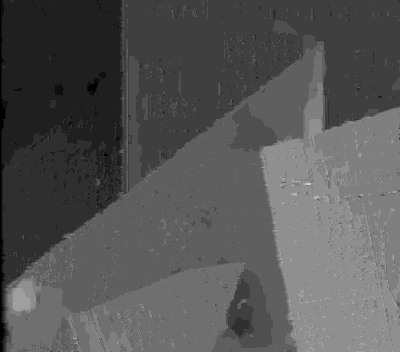
\includegraphics[width=\textwidth]{images/poster_pixel_based_stereo}
        \caption{$1'600$ ітерацій, $46$ хвилин, $\left| D \right| = 16$}
        \label{fig:poster:pixel}
    \end{subfigure}
    \caption{Карти глибин, отримані алгоритмом дифузії без сегментації зображення}
    \label{fig:result:pixel}
\end{figure}

На рисунку \ref{fig:result:superpixel} зображені карти глибин,
отримані за допомогою алгоритму дифузії з сегментацією зображення,
що описана в попередньому розділі дисертації,
з розміром комірок $5$ на $5$ пікселів.
Для кожного зображення вказано кількість ітерацій, зроблений алгоритмом дифузії,
час виконання всіх ітерацій, а також кількість міток $\left| D \right|$ в графі.
Отримані досить гладкі карти глибин,
однак видніються неточності на краях об'єктів.

\begin{figure}[h]
\centering
    \begin{subfigure}[t]{0.32\textwidth}
        \centering
        
\includegraphics[width=\textwidth]{images/cloth_superpixel_based_stereo}
        \caption{$100$ ітерацій, $19$ хвилин, $\left| D \right| = 40$}
        \label{fig:cloth:superpixel}
    \end{subfigure}
    \hfill
    \begin{subfigure}[t]{0.32\textwidth}
        \centering
        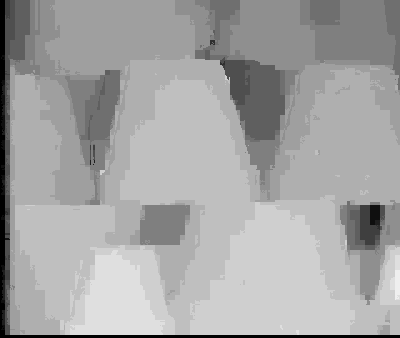
\includegraphics[width=\textwidth]{images/pots_superpixel_based_stereo}
        \caption{$450$ ітерацій, $15$ хвилин, $\; \left| D \right| = 16$}
        \label{fig:flowerpots:superpixel}
    \end{subfigure}
    \hfill
    \begin{subfigure}[t]{0.32\textwidth}
        \centering
        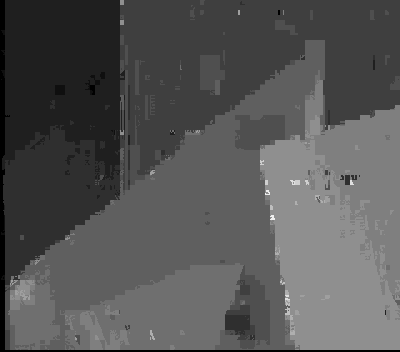
\includegraphics[width=\textwidth]{images/poster_superpixel_based_stereo}
        \caption{$400$ ітерацій, $14$ хвилин, $\; \left| D \right| = 16$}
        \label{fig:poster:superpixel}
    \end{subfigure}
    \caption{Карти глибин, отримані алгоритмом дифузії після сегментації зображення}
    \label{fig:result:superpixel}
\end{figure}

Для порівняння на рисунку \ref{fig:result:dynamic}
наведені карти глибин,
отримані з тими самими штрафними функціями
та значеннями параметрів за допомогою динамічного програмування,
де для кожного рядка зображення карта глибин шукається незалежно.
Хоча алгоритм і працює дуже швидко,
на отриманих картах глибин чітко видно горизонтальні лінії,
які є результатом того, що всі рядки зображення обробляються незалежно.
Таким чином, не алгоритм не враховує гладкість об'єктів.
Даний метод описано в першому розділі дисертації.

\begin{figure}[h]
\centering
    \begin{subfigure}[t]{0.32\textwidth}
        \centering
        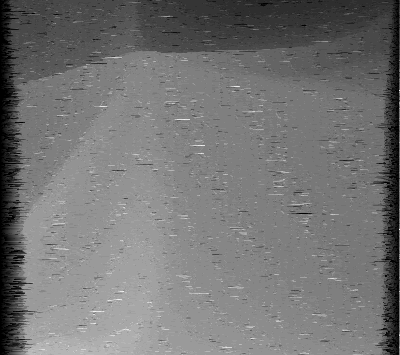
\includegraphics[width=\textwidth]{images/cloth_dynamic_result}
        \caption{$1.825$ секунди}
        \label{fig:cloth:result:dynamic}
    \end{subfigure}
    \hfill
    \begin{subfigure}[t]{0.32\textwidth}
        \centering
        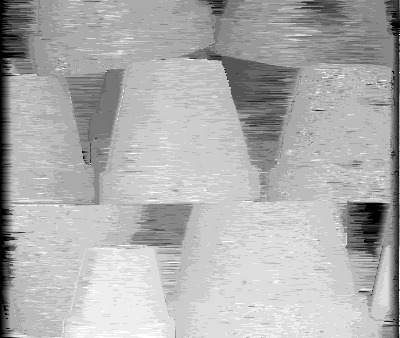
\includegraphics[width=\textwidth]{images/pots_dynamic_result}
        \caption{$0.792$ секунди}
        \label{fig:flowerpots:result:dynamic}
    \end{subfigure}
    \hfill
    \begin{subfigure}[t]{0.32\textwidth}
        \centering
        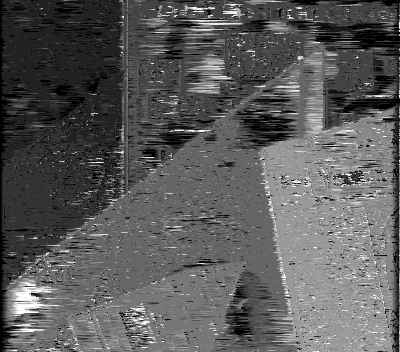
\includegraphics[width=\textwidth]{images/poster_dynamic_result}
        \caption{$0.83$ секунди}
        \label{fig:poster:result:dynamic}
    \end{subfigure}
    \caption{Карти глибин, отримані за допомогою динамічного програмування}
    \label{fig:result:dynamic}
\end{figure}

На рисунку \ref{fig:ground:truth}
наведені істинні синтезовані карти глибин,
надані разом за набором стереопар.

\begin{figure}[h]
\centering
    \begin{subfigure}[t]{0.32\textwidth}
        \centering
        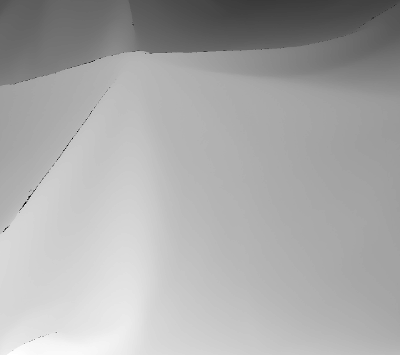
\includegraphics[width=\textwidth]{images/cloth_ground_truth}
        \caption{Тканина (Cloth1)}
        \label{fig:cloth:ground:truth}
    \end{subfigure}
    \hfill
    \begin{subfigure}[t]{0.32\textwidth}
        \centering
        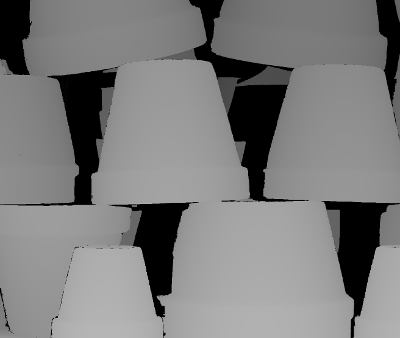
\includegraphics[width=\textwidth]{images/pots_ground_truth}
        \caption{Квіткові горщики (Flowerpots)}
        \label{fig:flowerpots:ground:truth}
    \end{subfigure}
    \hfill
    \begin{subfigure}[t]{0.32\textwidth}
        \centering
        
\includegraphics[width=\textwidth]{images/poster_ground_truth}
        \caption{Плакат (Poster)}
        \label{fig:poster:ground:truth}
    \end{subfigure}
    \caption{Істинні карти глибин}
    \label{fig:ground:truth}
\end{figure}

Алгоритм був реалізований на мові програмування Rust.
В ході роботи був використаний комп'ютер з процесором
Intel(R) Core(TM) i5-7400 і ОЗП DDR4 2133MHz.

\section{Покращення карти глибин}

Карти глибин, отримані алгоритмом дифузії не є такими гладкими,
як ідеальні карти глибин.
Для підвищення гладкості карт глибин та позбавлення від артефактів
після застосування алгоритмів стереобачення
часто використовують згладжуючі фільтри та інші методи обробки карти глибин.
Приклад одного з методів покращення карти глибин \cite{refinement}
наведений на рисунку \ref{fig:refinement}.
В даному методі для кожного пікселя розглядається
віконце певного розміру з центром в цьому пікселі.
Значення зсуву для даного пікселя перераховується шляхом голосування
з використанням сусідніх пікселів.
Далі використовується медіанний фільтр для згладжування зображення.
Він прибирає імпульсний шум, позбавляючи карту глибин від деяких артефактів.

\begin{figure}[h]
  \centering
  \begin{subfigure}[t]{0.45\textwidth}
      \centering
      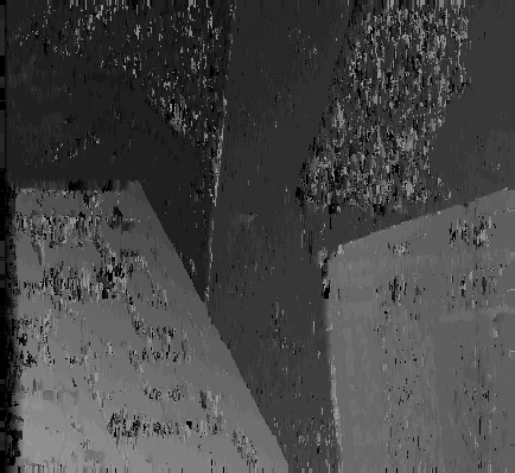
\includegraphics[width=\textwidth]{images/refinement_initial}
      \caption{Початкова карта глибин}
  \end{subfigure}
  \hfill
  \begin{subfigure}[t]{0.45\textwidth}
      \centering
      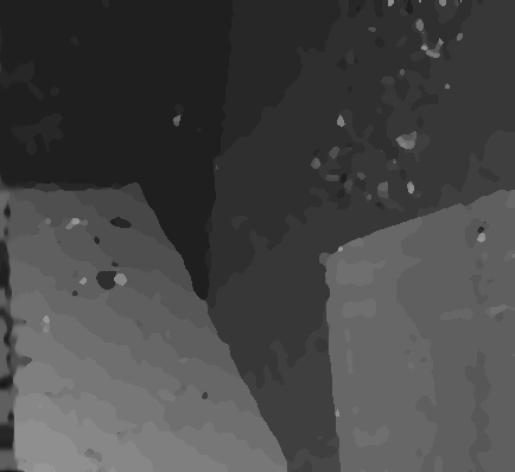
\includegraphics[width=\textwidth]{images/refinement_result}
      \caption{Покращена карта глибин}
  \end{subfigure}
  \caption{Приклад роботи одного з методів покращення карти глибин.
           Зображення взяті зі статті \cite{refinement}}
  \label{fig:refinement}
\end{figure}

\section{Штрафні функції}

В якості штрафної функції для вершин $f$
в даній роботі використовувався модуль різниці
інтенсивностей відповідних пікселів на двох зображеннях
\begin{equation*}
    f_{\left(x, y \right)} \left( d \right) =
    \left| L \left(x, y \right) - R \left(x - d, y \right) \right|,
\end{equation*}
$\left(x, y \right) \in T$, $d \in D$,
а в якості штрафної функції для дужок $g$~---~модуль різниці вибраних зсувів
$d \in D$ та $d' \in D$ в сусідніх об'єктах графу
\begin{equation*}
    g_{\left(x, y \right), \left(x', y' \right)} \left(d, d' \right) =
    \alpha \cdot \left| d - d' \right|,
\end{equation*}
де $\left(\left(x, y \right), \left(x', y' \right) \right) \in \mathcal{N}$,
а $\alpha = 1.4$~---~коефіцієнт згладжування,
підібраний експериментальним шляхом.
В попередньому розділі вказано, що
$\left| d - d' \right|$~---~субмодулярна функція від величин
$d, d' \in D$.
Після домноження на константу $\alpha \in \mathbb{R}$
функція залишається субмодулярною,
що гарантує існування розмітки після розв'язання оптимізаційної задачі
алгоритмом дифузії.

\section{Додаткові обмеження}

Додатково були введені обмеження на можливі мітки в кожному об'єкті:
для об'єкта $\left( x, y \right) \in T$ з горизонтальною координатою $x$
не може бути обраний зсув $d \in D$, такий що $d > x$,
який би перевів горизонтальну координату пікселя у від'ємне число
$x - d < 0$ (рис.~\ref{fig:disparity:restriction:vertex}).
Дані обмеження були введені за допомогою штрафної функції $f$
\begin{equation*}
    f_{\left(x, y \right)} \left( d \right) =
    \begin{cases}
        \left| L \left(x, y \right) - R \left(x - d, y \right) \right|,
            & x \ge d, \\
        + \infty, & x < d.
    \end{cases}
\end{equation*}

\begin{figure}[h]
  \centering
  \includegraphics[width=0.9\textwidth]{images/disparity_restriction_vertex}
  \caption{Обмеження на вибір мітки в об'єкті.
           $L_j$ та $R_j$~---~рядок під номером $j$
           лівого та правого зображення відповідно.
           Допустимі зсуви $d \in \left\{0, 1, 2, 3 \right\}$
           для даного об'єкта $\left(i, j \right)$
           з горизонтальною координатою $i = 3$
           зображено чорними стрілками,
           недопустимі зсуви $d > 3$~---~червоною стрілкою}
  \label{fig:disparity:restriction:vertex}
\end{figure}

Також були накладені обмеження на зсуви в сусідніх об'єктах по горизонталі:
$d' \le d + 1$ (рис.~\ref{fig:disparity:restriction:edge}),
де $d \in D$~---~мітка в об'єкті $\left(x, y \right) \in T$,
$d'$~---~мітка в об'єкті
$\left(x', y' \right) \in \mathcal{N} \left(x, y \right)$,
такому що $x' = x + 1$.

\begin{figure}[h]
  \centering
  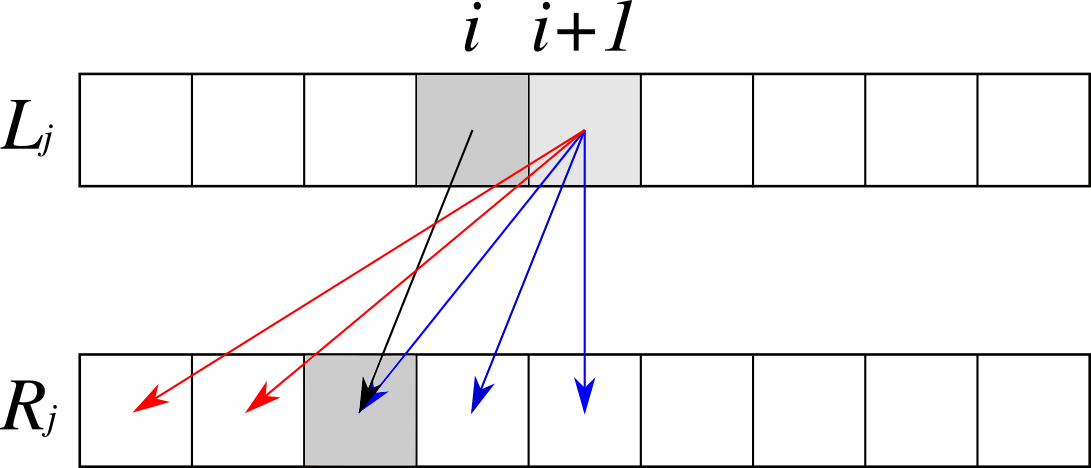
\includegraphics[width=0.9\textwidth]{images/disparity_restriction_edges}
  \caption{Обмеження на вибір міток в сусідніх об'єктах по горизонталі.
           $L_j$ та $R_j$~---~рядок під номером $j$
           лівого та правого зображення відповідно.
           Чорною стрілкою позначено обраний зсув $d \in D$ для об'єкту
           $\left(i, j \right)$.
           Синіми стрілками позначені допустимі зсуви $d'$
           для об'єкта $\left(i + 1, j \right)$, такі що $d' \le d + 1$,
           недопустимі зсуви $d' > d + 1$ позначено червоними стрілками}
  \label{fig:disparity:restriction:edge}
\end{figure}

% TODO: one image with different cell sizes comparison

\section*{Висновки до розділу 4}
\addcontentsline{toc}{section}{Висновки до розділу 4}

% TODO: add conclusions
